%########################################################################################
\chapter{Introduction} \label{Introduction} 
%########################################################################################

\clearpage

%========================================================================================
\section{Aflatoxins in the Food Production Chain} \label{subchap:AFs_introduction}
%========================================================================================

%----------------------------------------------------------------------------------------
\subsection{Aflatoxins: The Hidden Danger in Foods} \label{subchap:mycotoxins}
%----------------------------------------------------------------------------------------

Mycotoxins, produced as secondary metabolites by certain anamorphic fungal species, are natural contaminants in various food commodities, capable of causing disease and death in humans and animals upon consumption \citep{bennett2003clinical}. It is assumed that about 60 - 80\% of the global food crops are contaminated with mycotoxins \citep{eskola2020worldwide}. Roughly, more than a thousand mold species have been identified, of which more than 500 produce mycotoxins that have been classified as potentially toxic to vertebrates \citep{haque2020mycotoxin}. Major mycotoxins or groups of mycotoxins occuring in food that affect human and animal health include aflatoxins (AFs), ochratoxins, trichothecenes, fumonisins, alternariol, patulin and citrinin and alternaria toxins. These fungal toxins are produced by species within the genera \textit{Alternaria}, \textit{Aspergillus}, \textit{Fusarium} and \textit{Penicillium}. 


Aflatoxins (AFs), a group of mycotoxins that are produced by several species of the genus \textit{Aspergillus}, are widely considered as the most relevant mycotoxins from a food safety point of view due to their widespread occurence and high toxicity to humans \citep{afsah2013review, jallow2021worldwide}. To date, more than 20 aflatoxin molecules have been identified, with aflatoxin B1 (AFB1) exhibiting the highest toxicity to animals and humans \citep{ismail2018aflatoxin}. In addition to aflatoxin B1, the aflatoxins B2 (AFB2), G1 (AFG1), and G2 (AFG2),  as well as the derivative M1, which is primarily found in milk, are also of toxicological concern \citep{caceres2020aflatoxin, haque2020mycotoxin}. All aflatoxins are derivatives of dihydrofurancoumarins and share a common polycyclic structure derived from a coumarin nucleus linked to a bifurano system \citep{abrehame2023aflatoxins, nazhand2020characteristics}. They can be categorized into two chemical groups based on the binding to the dihydrofurancumarin structure: the difurocoumarocyclopentenone series (e.g., AFB1, AFB2, AFB2A, AFM1), characterized by the linkage to a pentanone ring, and the difurocoumarolactone series (e.g., AFG1, AFG2), characterized by the linkage to a lactone ring (Figure \ref{fig:Aflatoxins_structures_portrait}, \cite{abrehame2023aflatoxins, nazhand2020characteristics}). In addition, AFs can be further divided into AFs with (AFB1, AFB2, AFM1) and without (AFB2, AFG2, AFB2a) a double bond in the 8,9-position in the bifurano system \citep{abrehame2023aflatoxins}. 

%++++++++++++++++++++++++++++++++++++++++++++++++++++++++++++++++++++++++++++++++++++++++
\begin{figure}[ht!]
	\centering
	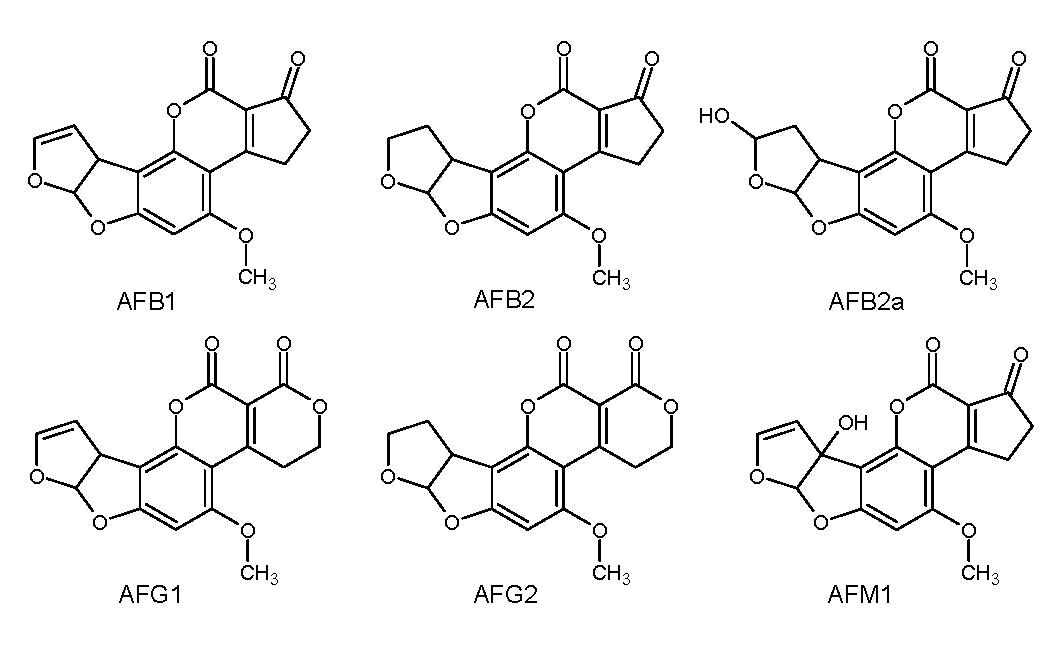
\includegraphics[width=1\textwidth]{figures/aflatoxins_structures_portrait.pdf}
	\decoRule
	\captionsetup{labelfont=bf, justification=justified, singlelinecheck=false, width=1\textwidth} 
	\caption{Structures of major important aflatoxins: aflatoxin B1 (AFB1), aflatoxin B2 (AFB2), aflatoxin B2a (AFB2a), aflatoxin G1 (AFG1), aflatoxin G2 (AFG2) and aflatoxin M1 (AFM1).}
	\label{fig:Aflatoxins_structures_portrait}
\end{figure}
%++++++++++++++++++++++++++++++++++++++++++++++++++++++++++++++++++++++++++++++++++++++++

%----------------------------------------------------------------------------------------
\subsection{Aflatoxin Occurrence in the Food Production Chain: Global Distribution and Geographical Variations} \label{subchap:occurence}
%----------------------------------------------------------------------------------------

Aflatoxin contamination is prevalent in various crops and regions worldwide, however, certain crops and conditions are more susceptible to AFs contamination. In general, oil- and starch-rich crops grown in (sub)tropical regions are the most susceptible to \textit{Aspergillus} infestation and aflatoxin contamination \citep{rushing2019aflatoxin, jallow2021worldwide}. Commodities that are frequently affected by aflatoxigenic fungi include cereals (wheat, sorghum, rice, acha, millet, guinea corn, corn), tree nuts (almond, pistachio, coconut, walnut), oilseeds (peanut, sunflower, cotton seeds, soybean, and sesame), spices (garlic, black pepper, coriander, turmeric, ginger, and chili peppers) \citep{awuchi2022mycotoxins}. The susceptibility of crops to fungal infestation and subsequent AFs production is influenced by a combination of environmental factors, crop-specific characteristics and the stage of food production chain and can already occurr "pre-harvest" in the field or "post-harvest" during storage, transport and processing (Figure \ref{fig:Food_chain}, \cite{jallow2021worldwide}).

%++++++++++++++++++++++++++++++++++++++++++++++++++++++++++++++++++++++++++++++++++++++++
\begin{figure}[ht]
	\centering
	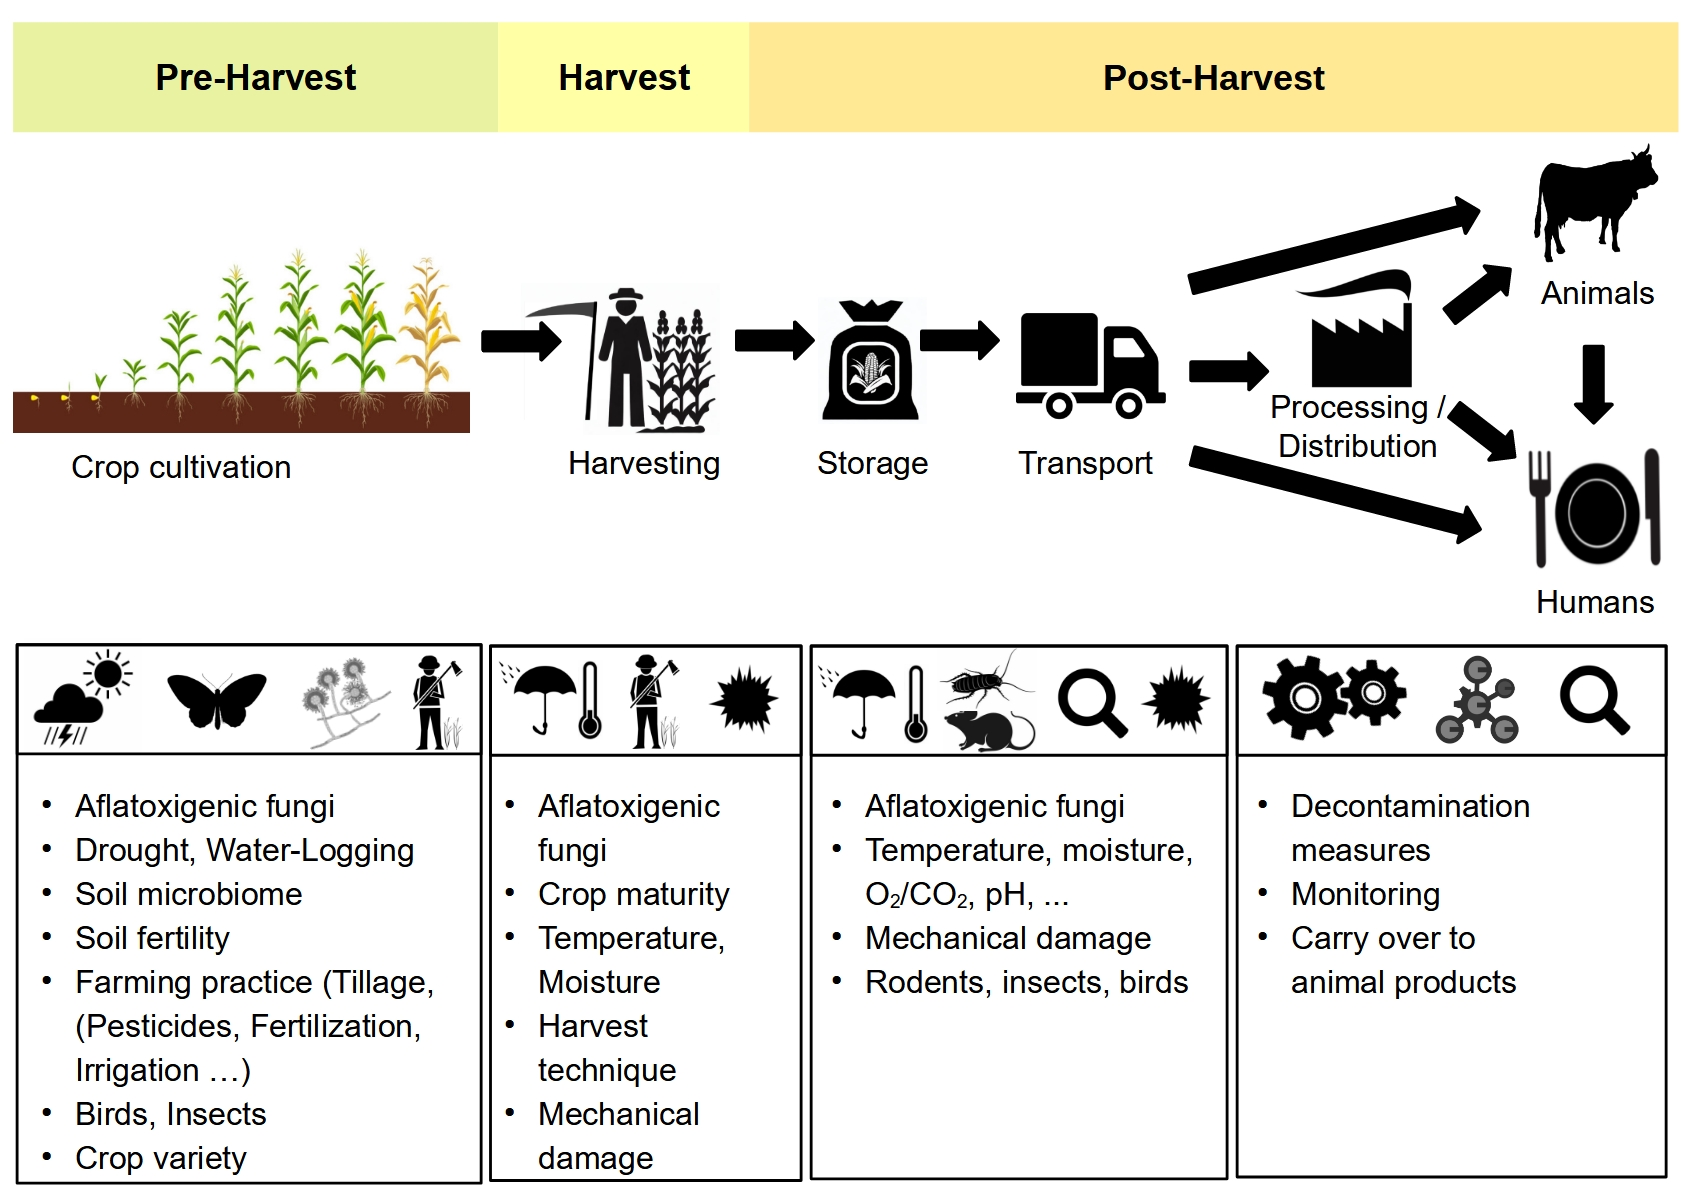
\includegraphics[width=1\textwidth,center]{figures/food chain.jpg}
	\decoRule
	\captionsetup{labelfont=bf, justification=justified, singlelinecheck=false, width=1\textwidth}
	\caption{Factors influencing aflatoxin occurrence throughout the food and feed production chain from pre-harvest to post-harvest stages.}
	\label{fig:Food_chain}
\end{figure}
\afterpage{\FloatBarrier}
%++++++++++++++++++++++++++++++++++++++++++++++++++++++++++++++++++++++++++++++++++++++++

Fungal growth and aflatoxin production are determined by chemical (pH, oxygen, carbon dioxide, nutrient substrate composition, pesticides), physical (temperature, moisture, water activity, mechanical damage) and biological factors (plant variety, seed quality, plant physiology, stress, pest insects, presence of compatible toxigenic fungi, soil microbiome) \citep{pleadin2019mycotoxins, bryden2012mycotoxin}. In the field, these conditions are primarily determined by weather and site conditions, as well as agricultural practices such as weeding, fertilization, pest control, irrigation, tillage, and harvesting techniques (Figure \ref{fig:Food_chain}). Conditions favoring pre-harvest contamination of crops such as peanuts and maize are high temperatures, insect damage and prolonged drought conditions \citep{bryden2012mycotoxin}. During and post-harvest stage, proper crop handling and processing, including adequate drying, clean and dry storage, and protection from rodents and insects, has a significant impact on aflatoxin fungal formation conditions (Figure \ref{fig:Food_chain}, \cite{kyei2021awareness}).

%++++++++++++++++++++++++++++++++++++++++++++++++++++++++++++++++++++++++++++++++++++++++
\begin{figure}[ht]
	\centering
	\includegraphics[width=\textwidth,center]{figures/aflatoxin_prevalence.jpeg}
	\decoRule
	\captionsetup{labelfont=bf, justification=justified, singlelinecheck=false, width=\textwidth}
	\caption{World maps showing the prevalence of AFs (sum of AFB1, AFB2, AFG1 and AFG2) in feed samples: (a) Percentage of positive samples; (b) Number of samples exceeding 5 \textmu{}g kg\textsuperscript{-1}; (c) Number of samples exceeding 20 \textmu{}g kg\textsuperscript{-1}. Areas filled in grey indicate data not available. The data used for plotting is sourced from \citet{gruber2019global}.}
	\label{fig:Aflatoxin_Prevalence}
\end{figure}
\afterpage{\FloatBarrier}
%++++++++++++++++++++++++++++++++++++++++++++++++++++++++++++++++++++++++++++++++++++++++

Developing countries from the (sub)tropics are particularly confronted with aflatoxin food contamination, due to the favorable (sub)tropical conditions for the growth and aflatoxin formation of these fungi and the limited access to control measures \citep{gbashi2018socio, nji2022six}. In a study by \citet{gruber2019global}, about 75,000 feed samples collected from 100 countries from 2008 to 2017 were analyzed for mycotoxins, including aflatoxins. The results showed a clear tendency towards a higher AFs prevalence in Southeast Asia (57.4 \%), South Asia (82.2 \%) and Sub-Saharan Africa (76 \%) and a much lower prevalence in Northern (5.9 \%) and Central Europe (12.7 \%) (Figure~\ref{fig:Aflatoxin_Prevalence}). Likewise the the number of samples exceeding 5 and 20  \textmu{}g kg\textsuperscript{-1} AFs are much higher in Southeast Asia (37.9 and 20.9 \%),  South Asia (61.1 and 41.1 \%) and Sub-Saharan Africa (59.1 and 38.5 \%) than in Northern (2.4 and 0.4 \%) and Central Europe (2.6 and 1.0 \%), respectively (Figure~\ref{fig:Aflatoxin_Prevalence}). 


These favorable (sub)tropical conditions for aflatoxigenic fungi result not only in higher prevalence, but also in significantly higher aflatoxin levels in agricultural products. Table \ref{table:Aflatoxin_food_levels} (Chapter \ref{Annex_chap1}) shows the reported aflatoxin contamination levels for various food commodities from countries in different geographical regions, adapted from the compilations by \citet{jallow2021worldwide} and \citet{ismail2018aflatoxin}. Corn and peanuts, major staple foods grown in (sub)tropical regions, are often associated with particularly high levels of aflatoxins \citep{ismail2018aflatoxin}. For example \textSigma AFs levels in the range of 10 \textsuperscript{3} \textmu g kg\textsuperscript{-1} were reported for cereals and peanuts in Uganda \citep{sserumaga2020aflatoxin}, Congo \citep{kamika2016occurrence}, Ethiopia \citep{mohammed2016aspergillus}, Nigeria \citep{oyedele2017mycotoxin}, Kenya \citep{sirma2016aflatoxin}, China \citep{wu2016aflatoxin} and Tunisia \citep{houissa2019multimycotoxin}.
Spices can also exhibit high levels of contamination, reaching concentrations in this range, as observed in Lebano \citep{el2019multimycotoxins}. In rare cases, \textSigma AFs concentrations above 10000 \textmu g kg\textsuperscript{-1} can be detected, as for example in infant preparations from Mexico \citep{chala2013natural}. Furthermore, due to the importance of corn as animal feed - about 55\% of corn production is used for this purpose - there is a strong link to the presence of aflatoxins in dairy products \citep{tolosa2021multi}. For instance, AFM1 concentrations of up to 4.5 \textmu g L\textsuperscript{-1} have been detected in milk samples from Kenya \citep{kuboka2019occurrence}. These significantly elevated contamination levels mentioned above have profound impacts on both human health and international trade.

%----------------------------------------------------------------------------------------
\subsection{Consequences of Aflatoxins: From Human Exposure to Global Trade} \label{subchap:AFs_consequences}
%----------------------------------------------------------------------------------------

The aflatoxin contamination level in foods and feeds, as well as the rate of consumption of the local population, largely determine the extent of human exposure to aflatoxins and the associated health effects \citep{jallow2021worldwide}. The average intake of aflatoxins by humans is estimated to be 10 to 200 ng kg\textsuperscript{-1} day\textsuperscript{-1}, with a total range of 0 to 30,000 ng kg\textsuperscript{-1} day\textsuperscript{-1} \citep{kaplan2003clinical, gong2016aflatoxin}. Given the high production and consumption rates of staple crops such as corn and peanuts, coupled with a high susceptibility to aflatoxin contamination, these crops are the primary source through which humans are exposed to aflatoxins. It is therefore no coincidence that the highest aflatoxin exposure is consistently reported from developing countries in (sub)tropical regions \citep{jallow2021worldwide}. In this regard, approximately 4.5 billion people in the developing world are at risk of chronic, uncontrolled exposure to AFs \citep{williams2004human, rushing2019aflatoxin, shephard2003aflatoxin, williams2004human}. Particular high exposure levels are reported for Sub-Saharan Africa and South-East Asia \citep{gong2016aflatoxin} such as Kenya (3.5-14.8 ng kg\textsuperscript{-1} day\textsuperscript{-1}), Swaziland (11.4-158.6 ng kg\textsuperscript{-1} day\textsuperscript{-1}), Mozambique (38.6-183.7 ng kg\textsuperscript{-1} day\textsuperscript{-1}), South Africa (16.5 ng kg\textsuperscript{-1} day\textsuperscript{-1}), The Gambia (4-115 ng kg\textsuperscript{-1} day\textsuperscript{-1}), China (11.7-2027 ng kg\textsuperscript{-1} day\textsuperscript{-1}), and Thailand (6.5-53 ng kg\textsuperscript{-1} day\textsuperscript{-1}) \citep{williams2004human}. Meanwhile, exposure levels in developed countries are much lower e.g. 2.7 ng kg\textsuperscript{-1} day\textsuperscript{-1} in the USA \citep{williams2004human} and 0.93–2.45 ng kg\textsuperscript{-1} day\textsuperscript{-1} in Europe \citep{jecfa2008sixty}.


Elevated exposure levels are of particular concern because AFs are considered one of the most potent mutagenic and carcinogenic substances known to date \citep{eskola2020worldwide}. The International Agency for Research on Cancer classifies AFB1 and natural aflatoxin mixtures of B, G, and M aflatoxins as group 1 carcinogens \citep{IARC2006}. Aflatoxins exhibit a toxicity profile where AFB1 is the most potent, followed by AFM1, AFG1, AFB2, and AFG2, with demonstrated acute toxicological and chronic hepatocarcinogenic effects in the liver due to their reactivity with DNA, RNA, enzymes, and proteins \citep{haque2020mycotoxin}. Chronic aflatoxicosis has been linked to hepatocellular carcinoma or liver cancer, suppress growth, modulate the immune system, and lead to malnutrition \citep{rushing2019aflatoxin, IARC2006, haque2020mycotoxin}. In addition, aflatoxicosis can exhibit potent synergistic effects with other factors contributing to liver cancers, such as malnutrition and infection with hepatitis B and C viruses, diseases that are highly prevalent in developing countries -- conditions highly prevalent in developing countries, with hepatitis incidences reaching about 20\% \citep{williams2004human}. Meanwhile, acute aflatoxicosis has resulted in symptoms such as abdominal pain, vomiting and edema \citep{eskola2020worldwide}. Especially in developing countries in (sub)tropical regions such as Kenya, China, India and Malaysia with favorable conditions for the growth and aflatoxin production of these fungi and limited access to control measures such as safe food storage, severe outbreaks of AFB1 contamination in food frequently occur, resulting in hundreds of deaths from acute aflatoxicosis \citep{azziz2005case, eskola2020worldwide, haque2020mycotoxin}. 


The impact of aflatoxin contamination in agriculture extends beyond public health, affecting  trade and economics in both developed and developing countries \citep{jallow2021worldwide}. In this regard, maize farmers in the US lose \$160 million annually due to AFs contamination \citep{wu2015global}, but losses are higher in developing countries, especially in sub-Saharan Africa, where they reach losses of \$450 million, representing 38\% of global agricultural losses due to aflatoxin \citep{gbashi2018socio}. Aflatoxins also lead to a significant decrease in agricultural trade between developed and developing countries \citep{wu2015global}, in part due to the discrepancy between these countries in terms of regulatory limits on the one hand and the prevalence of AFs on the other. In general, AFs regulation in non-tropical and industrialized countries that are less affected by AF problems are much stricter than in tropical and developing countries that are in heavily affected \citep{sirma2018impacts}. This discrepancy creates several problems for tropical countries facing the AF problem, such as sub-Saharan Africa. In these countries, economies are predominantly based on the commercialization of agricultural products \citep{matumba2015concentrating}. The economic importance of agricultural production, combined with a high susceptibility to AFs contamination, has a significant impact on the trade and economy of developing countries in the tropics mainly by reducing the value of the commodities offered for sale \citep{jallow2021worldwide}, e.g. by lowering prices, inspection fees, disposal fees, rejecting or treating lots at extra cost, compensating for claims, and the cost of sampling and analysis in the supply chain \citep{gbashi2018socio}. Typically, the main staple foods in these countries are also their most important cash crops \citep{nji2022six}. As a result, the best-quality crops with the least contamination that meet the standards of non-tropical importing countries are usually exported, leaving the poorer quality, more contaminated crops for local consumption or sale in the informal sector \citep{matumba2015concentrating, nji2022six}. This increases the likelihood of the local population consuming AFs contaminated foods \citep{udomkun2017mycotoxins, nji2022six}, with result in further economic costs i.e. cost of illness \citep{meijer2021aflatoxin}.


Contaminated crops unsuitable for sale in the informal food sector or for in-house consumption are often spread in the field for surface decomposition or buried in the soil as organic fertilizer \citep{fouche2020aflatoxins}. However, the fate and consequences of AFs in soil and on soil organisms that provide important ecological services remain unclear \citep{fouche2020aflatoxins}. Consequently, AFs contamination could go beyond health and trade issues,  potentially affecting soil health, agricultural productivity and food safety.

%----------------------------------------------------------------------------------------
\subsection{Regulation of Aflatoxins in Foods and Feeds: Efforts at Local and Global Scales} \label{subchap:globalregulation}
%----------------------------------------------------------------------------------------

%++++++++++++++++++++++++++++++++++++++++++++++++++++++++++++++++++++++++++++++++++++++++
\begin{figure}[ht]
	\centering
	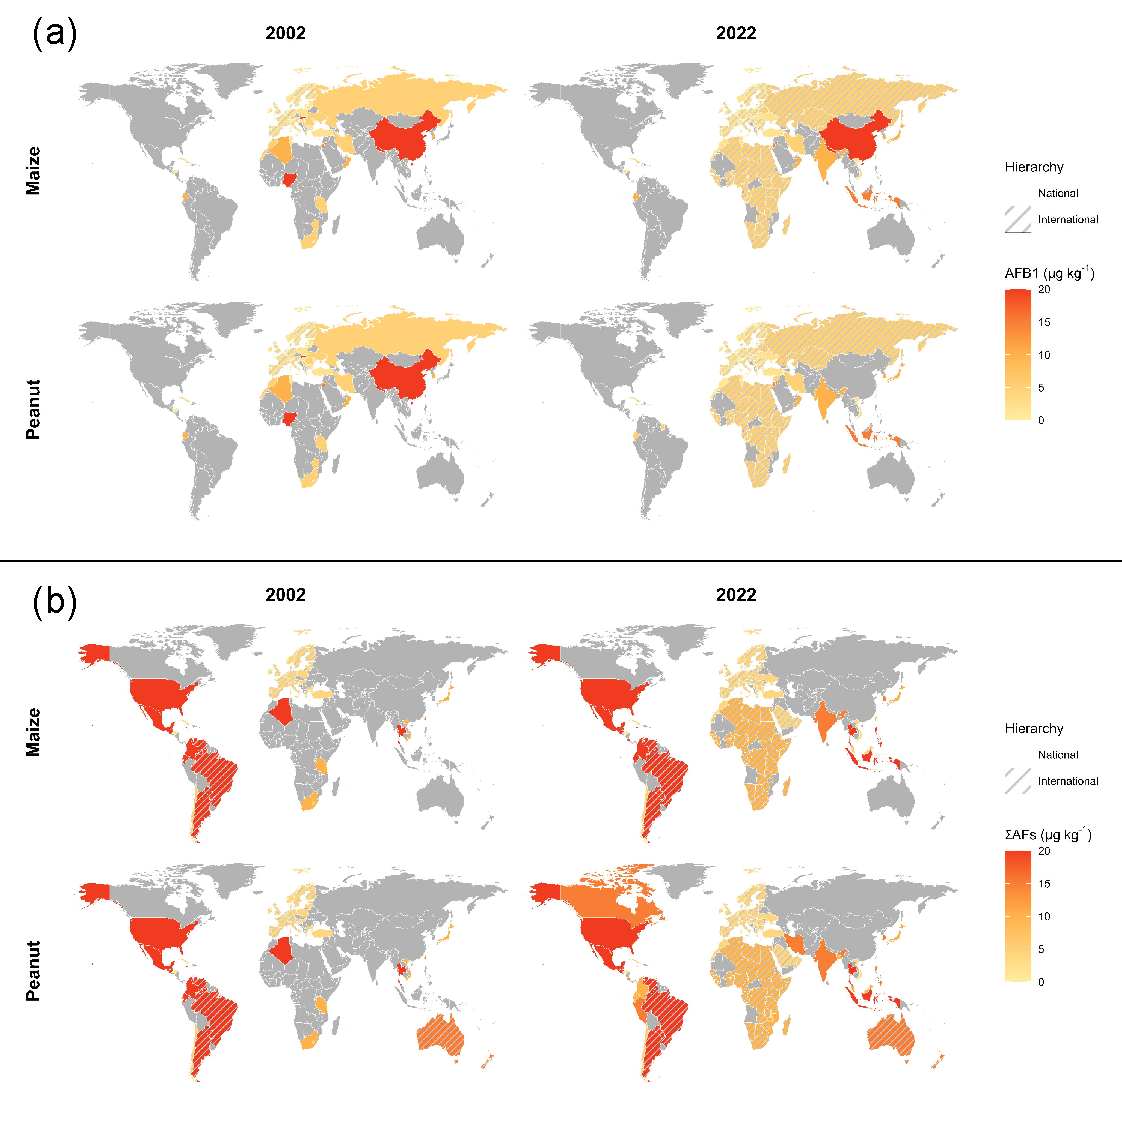
\includegraphics[width=1.15\textwidth,center]{figures/aflatoxin_regulation_limits.pdf}
	\decoRule
	\captionsetup{labelfont=bf, justification=justified, singlelinecheck=false, width=1.1\textwidth}
	\caption{World maps showing the regulation limits for AFB1 (a) and the sum of AFB1, AFB2, AFG1 and AFG2 (b) in maize and peanuts in the years 2002 and 2022. The polygons filled with a stripe pattern represent countries that have set limits for aflatoxin through international harmonized standards and those without a stripe pattern represent countries that have set their own national limits.}
	\label{fig:Aflatoxin_Regulation_Limits}
\end{figure} 
\afterpage{\FloatBarrier}
%++++++++++++++++++++++++++++++++++++++++++++++++++++++++++++++++++++++++++++++++++++++++

In order to protect humans and animals from the serious health effects of AFs, most countries have adopted strict regulations \citep{van2004worldwide}. Regulatory limits are established on sound risk assessments on the basis of toxicological and exposure data, as well as knowledge of the distribution of AFs concentrations within potentially susceptible commodities \citep{chilaka2022mycotoxin}. However, economic and political factors such as trade interests and adequate food supply also have an impact on the setting of local regulatory limits \citep{van2004worldwide}. In general, the maximum permissible values for AFs in foodstuffs are in the lower \textmu{}g kg\textsuperscript{-1} range \citep{van2004worldwide, sirma2018impacts}. In most countries, legal limits for the sum of the four major aflatoxins (AFB1, AFB2, AFG1 and AFG2) as well as the most toxic aflatoxin (AFB1) have been set at least for corn and peanuts due to their susceptibility and, at the same time, their importance as staple foods \citep{wu2013global}. A global survey conducted twenty years ago on behalf of the Food and Agriculture Organization of the United Nations (FAO) found that about 100 countries have specific regulations for AFs in various dairy products and feed items \citep{van2004worldwide}. The legal requirements differed strongly among the countries and regions (Figure~\ref{fig:Aflatoxin_Regulation_Limits}). While for Northern America, Southern America and Europe (inc. Russia) most countries implemented limits for AFB1 and/or the sum of AFs, there is a lack of regulation in Asian and African countries. Further, some free trade zones such as the EU, MERCOSUR, and Australia/New Zealand harmonized their limits. Although many countries do not have national or international legally binding limits for aflatoxins, it is important to know that many of these countries are members of the Codex Alimentarius Commission (CAC), which sets international standards, guidelines and codes of conduct to facilitate global trade and protect consumers. The CAC has established a standard for aflatoxins in peanuts (sum of AFs $\leq$ 15 \textmu{}g kg\textsuperscript{-1}), which, while not legally binding at the national level, can be considered a proxy regulation limit \citep{CAC1995}. A literature search on the situation of AF regulation in 2022 (Annex \ref{Annex_chap1}, Table~\ref{table:Aflatoxin_regulation}) revealed that an increasing number of countries have introduced limits either at national or internationally harmonized levels and that there is a general trend towards tightening AF limits, especially in African and Asian countries. By joining the European Union, several countries have adopted its particularly strict limits. Regionally harmonized aflatoxin limits have been introduced as a result of the formation of the Eurasian Customs Union (EACU), the East African Community (EAC), the African Organisation for Standardisation (ARSO) and the  Gulf Cooperation Council Standardization Organization (GSO). In addition, the number of Codex Alimentarius Commission member states increased between 2002 and 2022 from 168 to 189 (Figure~\ref{fig:Aflatoxin_Regulation_Limits}). Thus, the majority of countries in 2022 have some form of limits on AFs, either by setting national standards or by proxy. 


In non-tropical and developed countries where AF contamination is less prevalent, AF regulation levels are considerably more stringent compared to the regulations in tropical and developing nations, which are significantly more impacted by AF contamination \citep{sirma2018impacts}. For example, for the countries of the European Union the European Commission has defined some of the strictest limits with maximum permitted levels of 2 (AFB1) and 4 \textmu{}g kg\textsuperscript{-1} (sum AFB1, AFB2, AFG1, AFG2) and for maize and peanuts. On the other hand, the maximum levels set by the Ministry of Agriculture of the Republic of Indonesia are 15 (AFB1) and 20 \textmu{}g kg\textsuperscript{-1} (sum AFB1, AFB2, AFG1, AFG2) for maize and peanuts, respectively. These differences have significant implications for global trade and public health risks, as outlined in the previous chapter (Chapter \ref{subchap:AFs_consequences}). 


Current aflatoxin limits, designed primarily for formal markets, have limited ability to protect consumers in informal settings, particularly in subsistence agriculture, which is the predominant food production system in sub-Saharan Africa \citep{nji2022aflatoxins}. Therefore, it is important to take proactive measures to prevent aflatoxin contamination rather than relying solely on the effectiveness of limits. Such a preventive approach can protect consumers and effectively mitigate economic losses. Since AFs contamination can occur at various stages of the food production chain (Chapter \ref{subchap:occurence}), prevention include both pre- and post-harvest measures to ensure a comprehensive approach to controlling the risk of aflatoxin contamination.


%----------------------------------------------------------------------------------------
\subsection{Aflatoxin Prevention from Field to Fork: Integrated Approaches Along the Food Production Chain} \label{subchap:prevention}
%----------------------------------------------------------------------------------------

Aflatoxin control strategies rely on the knowledge of critical factors leading to increased growth and/or AF production of mold fungi (Figure \ref{fig:Food_chain}, Chapter \ref{subchap:occurence}). Based on sound experimental evidence, the Codex Alimentarius Comission has established several codes of practice for the prevention and mitigation of AF contamination in various crops, such as cereals \citep{CAC2003}, peanuts \citep{CAC2004}, tree nuts \citep{CAC2010}, figs \citep{CAC2008} and spices \citep{CAC2017} based on Good Agricultural Practice \citep{fao2003development}. These guidelines suggest management practices for all stages of the food production chain, including pre-harvest, harvesting and post-harvest stages.


In the pre-harvest stages, AF control strategies focus on improving plant health and impairing the growth and AF production of the fungi. The susceptibility of crops to fungal infection is closely related to their physiological condition, which can be influenced by various agricultural practices. The management practices recommended by the CAC to minimize AF contamination in the field can be summarized as follows: Use of certified seeds of resistant varieties that are free of toxic fungi, plowing under / destroying / removing of plant debris that may have served or potentially serves as substrate for aflatoxigenic fungi, timely planting to avoid heat and drought stress during seed development and maturation, avoidance of plant overcrowding by maintaining optimal plant densities, crop rotation, proper plant nutrition (fertilization and liming), avoiding drought stress (irrigation), controlling fungal vectors and plant pathogens including \textit{Asgergilli} and parasitic fungi other than \textit{Aspergilli} (fungicides), nematodes (nematocides), mites (acaricides), insects (insecticides) and weeds (herbicides). 


Recommended harvesting techniques are based on selecting harvesting conditions that reduce the risk of biological contamination. Firstly, appropriate harvest timing must be selected, which involves harvesting the crop when it has reached full maturity, ensuring acceptable moisture content, and prior to the onset of extreme weather conditions such as excessive heat, rainfall, or drought. In addition, functional and clean harvesting equipment should be used to allow timely harvesting, minimize physical damage to the harvested crop, and prevent the carryover of soil, dirt, dust, or contaminated plant material that could potentially serve as an inoculum for aflatoxigenic fungi. Any contact between the harvested crop and materials that may contain viable fungal structures should be avoided. Special attention should be paid to individual plants that have been damaged by pests or plant fractions with visible fungal contamination. These plants should be harvested separately to prevent rapid colonization by aflatoxigenic fungi during subsequent steps such as storage, transport and processing.


Post-harvest measures focus on preventing fungal invasion and/or creating conditions unsuitable for fungal growth and toxin formation. This includes avoiding piling, heaping, and storage of freshly harvested commodities with high moisture for extended periods of time. The crop should be dried as soon as possible after harvest in a manner that minimizes damage to the grain and maintains moisture levels lower than necessary for fungal growth during storage. In cases where immediate drying is not feasible, adequate aeration should be implemented. The drying, storage, and transport processes should take place in a clean, intact, protected, dry, and well-ventilated environment to protect the commodity against rain, dew, soil, pests, bird droppings, and other potential sources of contamination. Proper cleaning of the harvest is essential to remove damaged and immature plant material, as well as other foreign matter that may pose a risk of fungal infection. Continuous monitoring of the condition of stored and transported material is necessary to maintain acceptable temperature and moisture levels and minimize the presence of rodents and stored product pests, as these conditions can create favorable conditions for mold growth and AF production. The use of approved fumigants or insecticides may be appropriate for extended periods of transportation or storage.

Although soil is the natural habitat of AF producing fungi \citep{horn2003ecology, elmholt2008mycotoxins}, none of the proposed preventive measures specifically address soil as a conservation target. In fact, the impact of preventive measures on soil AF concentrations remains unknown. Certain actions, such as incorporation of plant residues by plowing, may potentially contribute to elevated AF input levels to soil \citep{fouche2020aflatoxins}.  Further, certain recommended management practices including fertilization, liming, irrigation, pesticide use can have negative effects on the integrity and functionality of the soil microbial communities \citep{tilman2002agricultural, sanaullah2020terrestrial}, potentially leading to changes in processes involved in the formation and dissipation of AFS. This, in turn, could affect the persistence of AFs in the soil and lead to ecological imbalances that potentially pose a threat to soil health. Therefore, soil has been largely neglected despite its central function in the context of AF prevention.



%========================================================================================
\section{Aflatoxins in the Soil Environment} \label{subchap:aflatoxins_in_soil}
%========================================================================================

%----------------------------------------------------------------------------------------
\subsection{Entry Pathways for Aflatoxins into the Soil} \label{subchap:entry}
%----------------------------------------------------------------------------------------

%++++++++++++++++++++++++++++++++++++++++++++++++++++++++++++++++++++++++++++++++++++++++
\begin{figure}[b!]
	\centering
	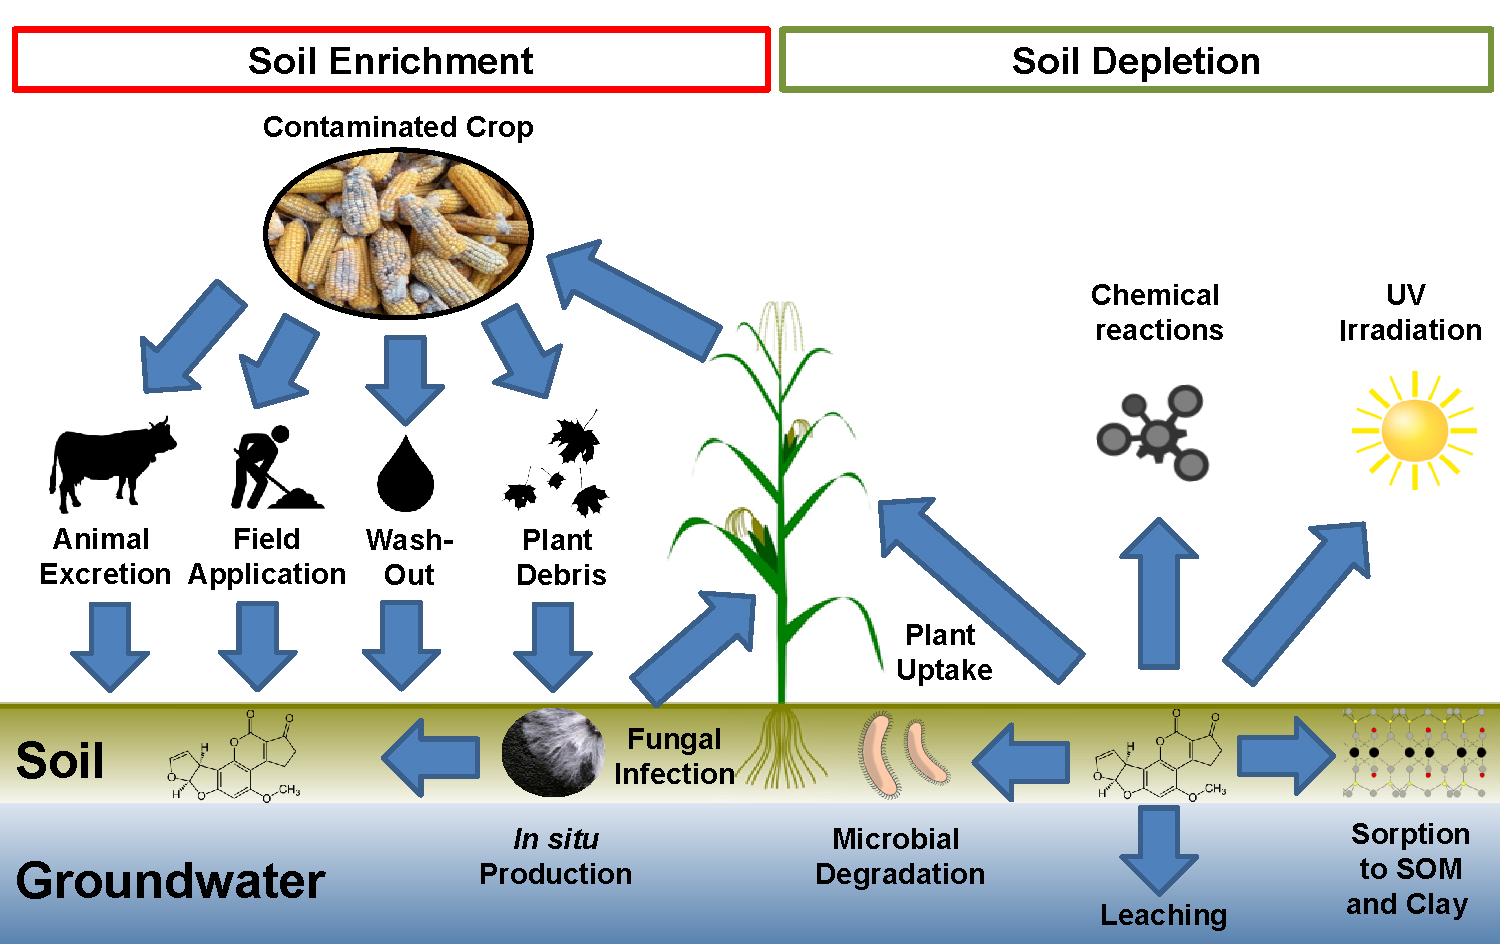
\includegraphics[width=1\textwidth,center]{figures/aflatoxin_pathways.pdf}
	\decoRule
	\captionsetup{labelfont=bf, justification=justified, singlelinecheck=false, width=1\textwidth}
	\caption{Aflatoxigenic fungi and aflatoxins in the soil environment: Possible entry pathways and degradation, sorption and transportation processes. Processes leading to soil enrichment with AFs are shown on the left side and processes leading to soil depletion are shown on the right side.}
	\label{fig:Aflatoxin_pathways}
\end{figure}
%++++++++++++++++++++++++++++++++++++++++++++++++++++++++++++++++++++++++++++++++++++++++

Natural entry pathways include \textit{in situ} aflatoxin production in soil and plant debris, rainfall-induced washoff from fungal-infested plant material, and moldy seeds and leaves shed by plants (Figure~\ref{fig:Aflatoxin_pathways}, \cite{elmholt2008mycotoxins, juraschek2022mycotoxins, fouche2020aflatoxins}). Anthropogenic activities such as livestock farming (animal excretion and manure application), planting with poor seed quality (moldy seeds) and incorporation of contaminated material (crop residues, moldy silage, waste kernels) can result in inputs of aflatoxigenic fungi and AFs into the soil  (Figure~\ref{fig:Aflatoxin_pathways}).  


The low water solubility of -3.5 to -0.4 log\textsubscript{10} mol L\textsuperscript{-1} and logK\textsubscript{OW} value of -0.7 to 1.8 suggest that  rainfall-induced washoff is a negligible pathway for AFs to enter the soil (Table~\ref{table:Aflatoxin_properties}). However, it should be noted that contaminated plant material may break off and fall to the ground due to the mechanical forces induced by rain, humans or animals. 


\citet{accinelli2008aspergillus} found that in soil, AFs are synthesized in in the range of 10\textsuperscript{2} (cobs containing grain), 10\textsuperscript{0} (leaves, stalks and cobs without grain) and 10\textsuperscript{-1} \textmu g kg\textsuperscript{-1} (soil). These results suggest that \textit{in situ} production in soil is rather neglible, whereas \textit{in situ} production in plant debris (in particular nutrient rich plant material) can be a significant source of AFs in soil. 

Studies from feeding trials have shown that mycotoxins from contaminated feed are transferred either as parent substance or metabolite to the urine and faeces of animals \citep{elmholt2008mycotoxins} and thus may enter the soil via manure. While for pig feeding trials with AFB1 contaminated feed, the excretion rates for AFB1 and AFM1 were on average 30 \% (77\% AFB1 + 23 \% AFM1) \citep{thieu2009zearalenone}, the excretion rates were rather negligible for cows with only 1.55\% (urine) and 2.79\% (faeces) \citep{allcroft1968excretion}. Thus, the excreta of certain livestock could be an important pathway for AFs to enter the soil.

\hfill

%++++++++++++++++++++++++++++++++++++++++++++++++++++++++++++++++++++++++++++++++++++++++
    \begin{table}[ht!]
    \footnotesize
        \begin{threeparttable}        
        \captionsetup{labelfont=bf, justification=justified, singlelinecheck=false, width=1\textwidth} 
        \caption{Physico-chemical properties and partition coefficients for the four main aflatoxins (AFB1, AFB2, AFG1, AFG2) and two main metabolites (AFB2a, AFM1). Property values represent the median of estimates from various models implemented in physical-chemical property estimation software (including OCHEM, EPISuite, ACD/Labs, and OPERA) \citep{tebes2018demonstration}. The individual estimates and models are given in Chapter \ref{Annex_chap1}.} 
\begin{tabular}{llllllll}  
	\toprule
	\textbf{Property}           & \textbf{Unit}                                    & \textbf{AFB1} & \textbf{AFB2} & \textbf{AFG1} & \textbf{AFG2} & \textbf{AFB2a} & \textbf{AFM1} \\
	\midrule
	Formula                     & -                                                & \ce{C17H12O6} & \ce{C17H14O6} & \ce{C17H12O7} & \ce{C17H14O7} & \ce{C17H14O7}  & \ce{C17H12O7} \\
	M                           & g mol\textsuperscript{-1}                        & 312.27        & 314.29        & 328.28        & 330.29        & 330.29         & 328.28        \\
	M\textsubscript{mi}         & g mol\textsuperscript{-1}                        & 312.06        & 314.08        & 328.06        & 330.07        & 330.07         & 328.06        \\
	HBA                         & -                                                & 6             & 6             & 7             & 7             & 7              & 7             \\
	HBD                         & -                                                & 0             & 0             & 0             & 0             & 1              & 1             \\
	
	
	T\textsubscript{b}          & °C                                              & 474           & 472           & 511           & 510           & 509            & 502           \\
	T\textsubscript{m}          & °C                                              & 207           & 230           & 230           & 217           & 217            & 214           \\
	log(P\textsubscript{v})     & mmHg                                             & -8.9          & -9.8          & -10.2         & -9.9          & -8.5           & -11.8         \\
	Log(c\textsubscript{max,w}) & mol L\textsuperscript{-1}                        & -3.1          & -2.9          & -3.5          & -2.8          & -2.6           & -2.5          \\
	Log(K\textsubscript{OW})    & -                                                & 1.2           & 1.4           & 1.8           & 0.7           & -0.4           & -0.2          \\
	Log(K\textsubscript{H})     & atm m\textsuperscript{3} mol\textsuperscript{-1} & -9.1          & -12.9         & -12.3         & -13.5         & -17.2          & -16.8         \\
	Log(K\textsubscript{OC})    & L/kg                                             & 1.9           & 1.9           & 1.8           & 1.8           & 1.2            & 1.3           \\
	\bottomrule
\end{tabular}
\label{table:Aflatoxin_properties}
            \begin{tablenotes}[flushleft]
                \setlength\labelsep{0pt}
                \footnotesize 
                %\itshape
                \item Formula = Empiric formula; M = Molar mass; M\textsubscript{mi} = Monoisotopic mass; HBA = Hydrogen Bond Acceptor Count; HBD = Hydrogen Bond Donor Count; T\textsubscript{b} = Boiling point; T\textsubscript{m} = Melting point; Log(P\textsubscript{v}) = Vapor pressure, logarithmic scale; Log(c\textsubscript{max,w}) = Water solubility, logarithmic scale; Log(K\textsubscript{OA}) = Octanol-Air-partitioning coefficient, logarithmic scale; Log(K\textsubscript{OW}) = Octanol-Water-partitioning coefficient, logarithmic scale; Log(K\textsubscript{H}) = Henry coefficent, logarithmic scale; Log(K\textsubscript{OC}) = Soil absorption coefficient, logarithmic scale. 
            \end{tablenotes}
        \end{threeparttable}
       % \end{adjustwidth}
    \end{table} 
%++++++++++++++++++++++++++++++++++++++++++++++++++++++++++++++++++++++++++++++++++++++++

%----------------------------------------------------------------------------------------
\subsection{Environmental Fate of Aflatoxins in Soil Systems} \label{subchap:dissipation}
%----------------------------------------------------------------------------------------

In soil, AFs may undergo various transformation, translocation and sorption processes (Figure~\ref{fig:Aflatoxin_pathways}) that depend strongly on the physicochemical properties of the soil and the functionality of the soil microbiome. However, experimental studies on the the environmental fate of AFs in soil are extremely scarce and mostly originate from laboratory experiments \citep{elmholt2008mycotoxins}. Despite a lack of experimental studies, predictions regarding certain soil processes can be made based on the physicochemical properties (Table~\ref{table:Aflatoxin_properties}). 

%----------------------------------------------------------------------------------------
\subsubsection*{Sorption and Transport} \label{subsubchap:sorption}
%----------------------------------------------------------------------------------------

The high boiling point of 472 - 511 °C, low vapor pressure of -11.8 to -8.5 log\textsubscript{10} mmHg and Henry partition coefficient of -17.2 to -9.1 log\textsubscript{10} atm m\textsuperscript{3} mol \textsuperscript{-1} suggests that AFs exist solely in the particulate phase and dissipation by volatilization is very unlikely (Table~\ref{table:Aflatoxin_properties}). 


Aflatoxins strongly sorb onto soil organic matter such as humic acids \citep{van2006vitro} with logK\textsubscript{OC} values ranging from 2.80 to 3.46 (experimentally derived, \citet{schenzel2012experimentally}) and from 1.2 to 1.8 L kg\textsuperscript{-1} (estimated, Table~\ref{table:Aflatoxin_properties}). \citet{goldberg1985aflatoxin} found that the sorption affinity of AFB1 to clay minerals was strongly dependant on clay mineral content and higher than that to soil organic matter. Moreover, the adsorption coefficient of AFB1 was about five times higher in a less humic silty clay loam  (0.6\% organic carbon, 37.8\% clay) than in a much more humic silt loam (2.9\% organic carbon, 33.6\% clay).


Due to their strong interaction with clay minerals and organic carbon combined along with their low water solubility (-3.5 to -0.4 log\textsubscript{10} mol L\textsuperscript{-1}), their mobility in water is restricted. \citet{goldberg1985aflatoxin} demonstrated a low leaching risk for various soils and found that AFB1 or its derivatives, AFB2 and AFG2, were retained in the top 20 cm of all soil types. The major part (80 to 92\%) of the AFB1 applied was retained within the top 2.5 cm of soil, and no AFs were detected in the leachate.


Since AFs are intermediate-polar substances (logK\textsubscript{OW} value of -0.7 to 1.8) compounds with low molecular weight of 312.27 to 330.29 g mol\textsuperscript{-1}, AFs have the potential to be taken up by plant roots and transported to aboveground plant parts. Plant uptake of AFs was documented for certain crops including lettuce \citep{mertz1981absorption}, maize \citep{mertz1980uptake}, peanut \citep{snigdha2013mechanism, snigdha2015transport}, sugarcane \citep{hariprasad2015natural} and soybean \citep{jones1980toxic} and several green leafy vegetables \citep{hariprasad2013natural}. While significant amounts of AFs in the range between 10\textsuperscript{0} and 10\textsuperscript{1} \textmu g kg\textsuperscript{-1} were accumulated during plant cultivation without soil, e.g. in coconut and hydroponic systems \citep{snigdha2013mechanism, snigdha2015transport, hariprasad2013natural}, only small amounts of AFs of less than 1\% were taken up by plants grown in soil contaminated with AFs \citep{mertz1980uptake}. 

%----------------------------------------------------------------------------------------
\subsubsection*{Biological Degradation} 
%----------------------------------------------------------------------------------------

Microbial degradation is considered a major important removal process for aflatoxins in soil \citep{fouche2020aflatoxins}. The degradation of AFs through microbial and enzymatic processes has been reported with half-lifes of few hours to days \citep{wu2009biological, verheecke2016microbial}. Studies were conducted in controlled environments such as bioreactors, liquid and agar cultures and media specific to the food matrix, thereby utilizing fungi from decaying wood \citep{alberts2009degradation, motomura2003purification}, microorganisms from soil contaminated with persistent pollutants \citep{teniola2005degradation, alberts2006biological}, microorganisms used in food processing \citep{megalla1982detoxification}, and microorganisms from the digestive tract \citep{kiessling1984metabolism, jones1996degradation}. These studies reported fast AFB1 dissipation rates, occurring within a few hours to days \textit{in vitro}. In soil, AFB1 was observed to dissipate at concentrations in the range between 10\textsuperscript{0} and 10\textsuperscript{4} \textmu g kg\textsuperscript{-1} within a week \citep{accinelli2008aspergillus, angle1980decomposition, angle1986aflatoxin}. So far, only mineralization has been quantitatively investigated in the context of AFB1 dissipation. \citet{angle1986aflatoxin} showed that mineralization is responsible for only a small fraction of the total dissipation of AFB1, with a 1.4 - 14\% mineralization occurring over a 112-day period. However, understanding of other processes that contribute to the dissipation of AFs in soil, such as volatilization, formation of bound residues, or their incorporation into microbial biomass, and how these processes are affected by soil properties is still limited.

%----------------------------------------------------------------------------------------
\subsubsection*{Abiotic Degradation} 
%----------------------------------------------------------------------------------------

Numerous physical and chemical processes are known to detoxify AFs in food matrices, such as treatment with UV light, organic acids, ammonia, sulfites, hydroxides and peroxides, among others \citep{pankaj2018review, piva1995detoxification, diao2015ultraviolet, peng2018current}. Aflatoxins released into the soil environment may also be exposed to these conditions, although empirical evidence for such abiotic degradation processes is currently lacking. However, agricultural practices suggested by the CAC (Chapter \ref{subchap:prevention}) e.g. fertilization, liming, tillage and biochemical transformation reactions can introduce or form reactive substances and create conditions in the soil that may ininiate abiotic degradation processes of AFs, similar to those observed in food matrices. Another aspect to be considered in degradation process in the soil is the texture and composition, as soil components such as clay minerals and humic substances may catalyze physicochemical degradation processes \citep{starr2017solvent,fripiat1974clays, birkel2002abiotic, garrido2010clays, wang2020transformation}. 

Finally, it should be considered that exposure to sunlight may occur when contaminated materials are on the soil surface or in plant debris. Aflatoxins absorb light in the UV range, and treatment of contaminated foods and feeds with UV light has been reported as an efficient treatment strategy to reduce AFs levels within a very short time i.e. with half-lives of only a few hours \citep{diao2015ultraviolet}. However, the abiotic degradation of aflatoxins in a soil exposed to UV light has not been studied so far, though photodegradation on soil surface may be a significant process for AFs degradation in the soil environment.


%----------------------------------------------------------------------------------------
\subsection{Aflatoxins and their Potential Impact on Soil Health} \label{subchap:soilhealth}
%----------------------------------------------------------------------------------------

%----------------------------------------------------------------------------------------
\subsubsection*{Soil Health and Importance of the Soil Microbiome} \label{subsubchap:soilhealth_definitions}
%----------------------------------------------------------------------------------------

Healthy soils perform crucial ecosystem functions, including water regulation, nutrient cycling, habitat provisioning, functioning as an environmental buffer or filter medium, carbon sequestration, support plant growth, providing physical stability and support, as well as contribute to resistance and resilience of terrestrial ecosystems \citep{maikhuri2012soil, lehmann2020concept, doran2000soil}. 
Understanding the key characteristics of soil health is essential for managing soils in a way that supports healthy plant growth and a diverse array of soil organisms \citep{lehmann2020concept}. Soil health indicators are classified as physical, chemical or biological. However, the boundaries between these categories are often blurred because many properties are due to multiple processes. For example, plant available phosphate is considered a chemical indicator, but it mainly results from microbial mineralization and plant uptake, which are biological processes \citep{lehmann2020concept}. The multifunctionality and diversity of soil requires multiple indicators to be quantified and integrated into an index. Soil microorganisms deserve special attention in this context. Soil microbial communities are involved in the provision of resources such as food, water, fiber, fuel, genetic resources, chemicals, medicines, and pharmaceuticals. By producing enzymes, soil microorganisms are the main drivers of decomposition of organic matter \citep{hattenschwiler2005biodiversity, prasad2021soil}, as well as secondary metabolites such as mycotoxins \citep{juraschek2022mycotoxins}, xenobiotic substances, such as pesticides \citep{parte2017microbial}. They are present in vast quantities, have high cumulative weight and activity, and meet most requirements to serve as valuable indicators of soil health \citep{sacca2017ecosystem}: They are sensitive to land management practices and environmental changes ("sensitive" criteria), exhibit a strong relationship with soil functions ("relevant and conceptual" criteria), and effectively illustrate the direct cause-and-effect relationship between land management decisions and plant health and productivity ("informative and interpretational" criteria) and are easily understood by land managers and are simple and inexpensive to measure ("effective and practical" criteria) \citep{sacca2017ecosystem, doran2000soil}.




The most extensively studied microbial parameters for soil health assessment to date primarily include microbial biomass, respiration rates, and growth characteristics observed on agar media. However, assessment of microbial biomass and activity may not be sufficient to evaluate environmental change, as significant shifts in microbial community structure have been observed without concomitant changes in microbial biomass and activity \citep{joergensen2006methods, fliessbach2004short}. In order to  fully understand the potential impact land management practices and environmental changes on soil health, it is important to investigate other microbial endpoints that are capable in reflecting more complex processes and functions in soil \citep{joergensen2006methods}. One approach for evaluating the physological and/or taxonomical structure of the microbial community is through the use of biomarkers such as the Phospholipid-Fatty-Acid-Analysis (PLFA) or molecular genetic measures such as amplicon sequencing and quantitative PCR with primers specific to certain taxa or functional groups. Changes in the physiological and functional state of the microbiome can be evaluated via enzymatic or respiration induced by readily avaiable substrates such as glucose. By extending substrate-induced respiration to multiple, structurally diverse substrates, utilization patterns of carbon sources can be determined, providing valuable insights into the ability of the soil microbiome to metabolize carbon sources of varying origins and structural complexity \citep{campbell2003rapid, chapman2007assessing}. Furthermore, microbial and ecophysiological ratios can be calculated from biomass, activity and nutrient properties to detect microbial stress and changes in the composition or physiological state of the microbial community \citep{joergensen2006methods, blagodatskaya2013active}.

%----------------------------------------------------------------------------------------
\subsubsection*{Ecological Function of Aflatoxins in the Soil and Implications for the Soil Microbiome} \label{subsubchap:soilhealth_threat} 
%----------------------------------------------------------------------------------------

Aflatoxigenic fungi do naturally occurr in soil and plant residues as their natural habitat \citep{horn2003ecology, jaime2004aspergillus, orum1997spatial, accinelli2008aspergillus}. The major part of the life cycle of these fungi takes place in the soil as they do not only colonize living plant tissue, but also grow saprophytically on organic residues in the soil \citep{abbas2009ecology}. These residues serve as a reservoir for the fungus, allowing it to overwinter, and under favorable conditions resume growth with the potential to infest plants and crops  \citep{horn2003ecology, abbas2009ecology}. In subtropical regions, aflatoxin-producing fungi and AF are natural components of soil ecosystems. To maintain a stable equilibrium in this ecosystem over the long term, there must be a balance between the natural production of AFs and their depletion. However, anthropogenic activities such as the disposal of contaminated crop residues in the field or livestock rearing can lead to additional inputs of aflatoxin-producing fungi and aflatoxins that far exceed natural levels (Chapter \ref{subchap:entry}). This form of anthropogenic input could disturb the natural balance of inputs and outputs, altering both the concentration and duration of exposure of the soil microbiome to aflatoxins \citep{fouche2020aflatoxins}. However, to determine if there is a potential threat to soil health, it is necessary to understand the ecological role of aflatoxins for the producing fungus and the potential impact on other microorganisms. 


Aflatoxins are secondary metabolites and their production is therefore not constitutive, but depends on environmental conditions \citep{carter2013aflatoxins}. During establishment and growth, aflatoxigenic fungi compete for resources with other living organisms in the soil. Therefore, aflatoxin production may be a protective response to microbial competition or predation, though empirical evidence for this function in the soil environment is limited. The presence of high AF concentrations in fungal structures that enter the soil, i.e., sclerotia, conidia spores and hyphae in infected plant material \citep{wicklow1983intrafungal}, however, suggests a protective measure by the fungus against predators and competitors during soil invasion. Furthermore, the presence of soil microbes, such as Gram-positive and Gram-negative bacteria, yeasts, and filamentous fungi, was found to enhance the \textit{in vitro} production of AFs \citep{weckbach1977aflatoxin, cuero1987stimulation, type1980interference}. However, other studies have reported different results, with the presence of filamentous fungi and Gram-positive bacteria not affecting, reducing, or completely inhibiting AF production \citep{weckbach1977aflatoxin, type1980interference}. Single species toxicity tests performed \textit{in vitro} on agar plates supplemented with AFB1 (30 and 100 mg L\textsuperscript{-1}) showed growth inhibition for some Gram-positive bacteria, including Bacillus, Nocardia, Clostridium, and Streptomyces \citep{burmeister1966survey, arai1967antimicrobial}. No effects on growth were observed for other common Gram-positive and Gram-negative bacteria, fungi, algae, and protozoa. Such selective growth inhibition effects could potentially reduce the competitiveness of the affected microbes within a soil microbial community, alter the community structure of the soil microbiome, and compromise the soil functions provided by these microorganisms. In a study by  \citet{angle1981aflatoxin}, the whole soil microbiome of a silt loam soil were isolated and then cultivated on AFB1 supplemented agar media (1-10,000 \textmu g L\textsuperscript{-1}). At a concentration of 10,000 \textmu g L\textsuperscript{-1}, AFB1 caused a 38\% reduction in the number of fungi and a 34\% reduction in the number of bacteria and actinomycetes, compared to the control.


However, all these studies were performed under optimised \textit{in vitro} conditions without considering soil as an environmental matrix. Although \textit{in vitro} studies provide key evidence on specific responses, they may not be representative of complex environmental systems since other influencing external factors are excluded \citep{drott2019fitness}. In addition, less than 1\% of the total microbiome can be cultured on agar media \citep{pham2012cultivation}. Furthermore, relatively high concentrations of aflatoxins are often used in \textit{in vitro} bioassay studies. The environmental media contaminated with AFs are likely usually much lower. For example, AFs concentrations ranging from 10\textsuperscript{-2} and 10\textsuperscript{2} \textmu g kg\textsuperscript{-1} have been reported for agricultural soils and crop residues \citep{accinelli2008aspergillus}. In this regard, \citet{drott2019fitness} investigated the fitness of aflatoxigenic and nonaflatoxigenic isolates of \textit{Aspergillus flavus} via quantitative PCR in soil microcosms. They found that aflatoxigenic isolates had lower fitness in natural soils across different temperature regimes (25, 37, 42 °C) and the addition of aflatoxin (500 \textmu g kg\textsuperscript{-1}) to the soils did neither affect \textit{A. flavus} growth nor the species richness of the fungal and bacterial communities (assessed via amplicon sequencing). However, it should be noted that although no lethal effects occurred, the physiology of the microbiome may have been impaired, e.g. in enzymatic or respiratory activity. In this context, \citet{angle1981aflatoxin} artificially contaminated soil with AFB1 in a range of 1-10,000 \textmu g kg\textsuperscript{-1} and determined soil respiration rates and numbers of viable fungi, bacteria, and actinomycetes of the isolated soil microbiome. Dose-dependent negative effects on the number of viable microorganisms were observed two weeks after AFB1 treatment, which persisted for almost six weeks. In addition, the authors observed a significant reduction in the respiration rate of the entire soil microbiome at the highest AFB1 enrichment level of 10,000 \textmu g kg\textsuperscript{-1} compared to the control, while respiration at lower levels was not significantly different from the control. 


The influence of soil composition on the toxicity and bioavailability of AFs to the soil microbiome has not yet been systematically investigated. In soil there are structures such as humus and clay minerals that could bind aflatoxins (Chapter \ref{subchap:dissipation}) and thus reduce their bioavailability to microbes. Furthermore, other measures for soil health assessment such as carbon source utilization patterns and PLFA have not been widely applied in aflatoxin exposure studies. This may be due in part to the fact that previous studies on the effects of AFs on the soil microbiome were conducted prior to the availability of these methods. As a result, there is a gap in the knowledge regarding the microbial responses to AFs exposure using endpoints with higher complexity and resolution, which would enable a more comprehensive assessment of the ecological function of aflatoxins for the producing fungi and their implications for the soil microbiome and associated functions.


%----------------------------------------------------------------------------------------
\subsection{Status and Challenges in the Analysis of Aflatoxins in Soils} \label{subchap:analysis}
%----------------------------------------------------------------------------------------

Understanding the occurrence and fate of AFs in the environment requires the use of appropriate and reliable analytical techniques. These techniques should be applicable not only at the level of agricultural products, but also in relation to the preceding steps in the production of raw materials, especially the interactions between the plant and soil ecosystems. Therefore, reliable analytical tools for the detection and quantification of AF in soils are essential for a better understanding of the environmental fate and ecological relevance of AFs in the soil environment. While a large number of methods exist for the extraction and determination of AFs in food and plant matrices, there is a lack of methods for soils. 


Although previous studies reported contamination of soil with AFs ranging from 10\textsuperscript{-2} to 10\textsuperscript{1} \textmu g kg\textsuperscript{-1} \citep{accinelli2008aspergillus}, it is important to note that these values may not accurately represent real environmental concentrations due to the lack of systematic validation for the specific soils analyzed using the presented analytical method. So far, reported recoveries were generally very low or methods were not systematically validated (Table \ref{table:Aflatoxin_extraction}). Furthermore, exorbitantly high AFs concentrations of 10\textsuperscript{3} and 10\textsuperscript{5} \textmu g kg\textsuperscript{-1} were applied to soil for spike-recovery experiments, which may be far above natural occurring levels (Chapter \ref{subchap:entry}). 

%++++++++++++++++++++++++++++++++++++++++++++++++++++++++++++++++++++++++++++++++++++++++
\begin{table}[t!]
\footnotesize
%\centering
\begin{adjustwidth}{-0.04\textwidth}{0.15\textwidth}% adjust the L and R margins by 1 inch
\begin{threeparttable}
\hfuzz = 100pt
\captionsetup{labelfont=bf, justification=justified, singlelinecheck=false, width=1\textwidth} 
\caption{Previously described analytical procedures for the extraction of AFs from soil matrices.} \label{table:Aflatoxin_extraction}
\begin{tabular}{lllllll}
\toprule
\textbf{\begin{tabular}[c]{@{}l@{}}Extraction\\ technique\end{tabular}} & \textbf{\begin{tabular}[c]{@{}l@{}}Extraction \\ solvents\end{tabular}}   & \textbf{\begin{tabular}[c]{@{}l@{}}Extraction\\ procedure\end{tabular}}   & \textbf{\begin{tabular}[c]{@{}l@{}}Soil \\ type\end{tabular}} & \textbf{\begin{tabular}[c]{@{}l@{}}AFs range\\ (µg kg-1)\end{tabular}} & \textbf{\begin{tabular}[c]{@{}l@{}}Recovery \\ (\%)\end{tabular}} & \textbf{Reference}  \\
\midrule
SLE & \begin{tabular}[c]{@{}l@{}}\ce{H2O}:EtOAc \\ (1:3)\end{tabular}& \begin{tabular}[c]{@{}l@{}}overnight \\ shaking\end{tabular}  & silt loam & 10 \textsuperscript{1}   & NA & \citet{accinelli2008aspergillus}\\
SLE & ACE   & \begin{tabular}[c]{@{}l@{}}30 min \\ shaking\end{tabular} & silt loam & 10 \textsuperscript{4}   & 18 & \citet{angle1980decomposition}\\
SLE & \begin{tabular}[c]{@{}l@{}}\ce{CHCl3}, MeOH, \\ \ce{CHCl3}:MeOH \\ (80:20)\end{tabular} & NA& loam soil & 10 \textsuperscript{4} - 10 \textsuperscript{5} & \textless{}1   & \citet{mertz1981absorption}\\
\multirow{4}{*}{SLE}& \multirow{4}{*}{ACE}  & \multirow{4}{*}{\begin{tabular}[c]{@{}l@{}}saturation \\ with \ce{H2O}, \\ 5 min \\ blending\end{tabular}} & silt loam,& \multirow{4}{*}{10 \textsuperscript{3}}  & \multirow{4}{*}{70}& \multirow{4}{*}{\citet{goldberg1985aflatoxin}} \\
&   &   & sandy loam,   &   && \\
&   &   & clay loam,&   && \\
&   &   & silty clay loam   &   && \\
SFE & \begin{tabular}[c]{@{}l@{}}MeCN + \\ 2\% AcOH\end{tabular}& \begin{tabular}[c]{@{}l@{}}15 min \\ static time\end{tabular} & silt loam & 10 \textsuperscript{3}   & 72 & \citet{starr2008supercritical}   
\\
\bottomrule
\end{tabular}
\begin{tablenotes}[flushleft]
\setlength\labelsep{0pt}
\footnotesize 
%\itshape
\item SLE = Solid-liquid-extraction; SFE = Supercritical-fluid-extraction; EtOAc = Ethyl acetate; ACE = Acetone; MeOH = Methanol; AcOH = Acetic acid. 
\end{tablenotes}
\end{threeparttable}
\end{adjustwidth}

\end{table}
 
%++++++++++++++++++++++++++++++++++++++++++++++++++++++++++++++++++++++++++++++++++++++++


The challenges associated with the extraction  of AFs from may be attributed to the complex and heterogeneous nature of soil as an environmental matrix, the way AFs interact with soil fractions and the need for detection of trace amounts, making it difficult to apply general methods \citep{fouche2020aflatoxins}. In this context, soil organic carbon content and texture play a crucial role (Chapter \ref{subchap:dissipation}), as evidenced by previous studies indicating medium-strong interactions with soil organic matter \citep{schenzel2012experimentally, van2006vitro} and very strong interactions with clay minerals \citep{kang2016understanding, goldberg1985aflatoxin}. AFs exhibit strong H-bond acceptor properties with a H-bond acceptor counts of 6 - 7 and weak H-bond donor properties with a H-bond donor counts of 0 - 1 (Table \ref{table:Aflatoxin_properties}). Due to this strong H-bond acceptor properties, AFs strongly sorb to clay minerals via electron-donor–acceptor interactions between the two electron-rich carbonyl groups in the coumarin structure of the AFs and electron-deficient or positively charged species located at the negatively charged surface of clay minerals \citep{kang2016understanding}. Most solvents tested to date have been monopolar solvents that have weak H-bond acceptor properties (e.g., chloroform) or bipolar solvents (e.g., methanol) and thus may not have been able to effectively displace AFs from cation H-bond sites. Thus, it remains to be determined whether the use of solvents that have similar polarity and H-bond acceptor properties to aflatoxins can effectively overcome the strong interactions between aflatoxins and soil.


%========================================================================================
\section{Open Questions and Rationale of the PhD Project}
%========================================================================================

Currently, the study of aflatoxins primarily revolves around their potential to contaminate food and feed, rendering them unfit for human consumption and trade. This emphasis is evident in the extensive research conducted on aflatoxins and aflatoxigenic fungi, exploring their chemistry, human toxicity, and the factors contributing to their presence in food and feed, primarily during post-harvest stages \citep{fouche2020aflatoxins}. Meanwhile their relevance at pre-harvest stages as environmental micropollutants in their natural habitat, namely soil, remain largely unexplored. The environmental fate of aflatoxins in soil and the consequences of aflatoxin contamination for soil microorganisms that perform essential ecological functions remain unclear. The current limited knowledge of the occurrence, fate, and ecological consequences of aflatoxins in soil hampers the understanding of their environmental relevance and may impede the development of effective pre-harvest strategies to control aflatoxin contamination.


These knowledge gaps regarding aflatoxins in the soil are probably attributed to methodological challenges encountered in successfully extracting aflatoxins from soils. Although sorption to certain soil compartments, particularly organic matter \citep{schenzel2012experimentally} and clay minerals \citep{kang2016understanding}, is known to contribute significantly to the particularly strong interactions of AF with soil, it is not yet known how these interactions could be overcome to allow effective extraction of aflatoxins from soils. In this regard, it remains uncertain whether the particular strong electron-donor-acceptor interactions between aflatoxins and the positively charged layers of the clay minerals can be effectively counteracted by utilizing solvents with similar polarity and H-bond acceptor properties to the aflatoxins, such as acetonitrile. Overcoming these interactions in developing a suitable analytical method for the extraction of aflatoxins is an essential prerequisite for studying the occurrence and fate of AFs in the environment.


Despite a basic understanding of the pathways by which aflatoxins could possibly enter the soil (Chapter \ref{subchap:entry}), there is a notable lack of experimental evidence on their general occurrence and distribution in the field, as well as on their dependence on site conditions, soil properties, and agricultural practices. Although preventive measures to successfully control aflatoxin contamination of field crops prior to harvest are well documented, their effect on aflatoxin occurrence in the soil remains uncertain. This is relevant because if such pre-harvest measures have an impact on soil contamination, this could also have an impact on integrity and functionality of the soil microbiome and thus to soil health.


Although laboratory experiments conducted in the absence of soil have led to a general understanding of the mechanisms of aflatoxin degradation (Chapter \ref{subchap:dissipation}), the understanding of the fate of aflatoxins in their complex natural environment "soil", is still largely incomplete. In the limited number of studies conducted in soil, rapid dissipation has been observed \citep{accinelli2008aspergillus, angle1980decomposition, angle1986aflatoxin}, but the processes responsible for this dissipation in interaction with soil physicochemical properties and aflatoxin concentrations, remain poorly understood. Furthermore, although aflatoxins can be exposed to UV light via sunlight at pre-harvest stages, the extent to which photolytic degradation occurs in a soil matrix has not yet been tested. This is relevant as as this degradation process has the potential to be a key driver in the reduction of aflatoxins in soil, consequently influencing the overall equilibrium within the soil.


\textit{In vitro} studies conducted without soil have shown the toxicity of aflatoxins to specific isolated soil microbes (Chapter \ref{subchap:AFs_consequences}), but the potential implications for the soil microbiome, influenced by the soil matrix and available concentration, are not well understood. In addition, previous research primarily concentrated on general microbial endpoints, such as the effects of AFs on specific organism groups and their biomass and activity. However, these general biomarkers may not be sufficient to detect environmental changes, as significant changes in microbial community structure have been observed without concomitant changes in microbial biomass and activity. Such a microbial change at the community and physiology level has the potential to impair functions provided by the soil microbiome with unknown consequences for soil health and agricultural productivity. 


Summarizing, in this thesis, it is attempted to address the following open research questions:

%++++++++++++++++++++++++++++++++++++++++++++++++++++++++++++++++++++++++++++++++++++++++
\begin{itemize}
\item[(1)] How can the interactions between aflatoxins and soil sorption sites, namely clay minerals and organic carbon, be effectively overcome to enable the extraction of aflatoxins from soils? 
\item[(2)] What is the occurrence and distribution of aflatoxins in contaminated soils, and to what extent does this depend on soil properties and agricultural practices intended to control fungal infestation and mycotoxin contamination of crops at the preharvest stage?
\item[(3)] Which processes contribute to the dissipation of aflatoxins in soil, and how are they modulated by soil properties, especially clay content, and aflatoxin concentration? 
\item[(4)] How do aflatoxin contamination affect the soil microbiome and its associated functions, and to what extent are these effects modulated by soil properties? 
\end{itemize}
%++++++++++++++++++++++++++++++++++++++++++++++++++++++++++++++++++++++++++++++++++++++++


%========================================================================================
\section{Objectives, Hypotheses and Structure of the Thesis}
%========================================================================================

The main objective of this PhD project was to scrutinize the mechanisms and extent of the occurrence of aflatoxins in soil, the processes of their dissipation and their impact on the soil microbiome and associated soil functions, and how these relate to soil properties.
There is evidence that aflatoxins strongly interact with certain soil structures, in particular with clay minerals, affecting their mobility and availability. Therefore, I hypothesize that the clay content affect the processes of aflatoxin dissipation and the impact of aflatoxins on the soil microbiome and associated functions. Various effective pre-harvest prevention measures have been reported to control aflatoxin contamination in crops, involving inhibiting aflatoxin-producing fungi growth and production, controlling fungal vectors like insects, and enhancing plant health to reduce susceptibility to fungal infection. As a result, I hypothesize reduced aflatoxin soil levels in fields where these measures are implemented. To address these hypotheses, the structure of the PhD thesis encompasses four parts, comprising laboratory and field experiments (Figure~\ref{fig:Thesis_structure}). 

%++++++++++++++++++++++++++++++++++++++++++++++++++++++++++++++++++++++++++++++++++++++++
\begin{figure}[ht!]
\centering
 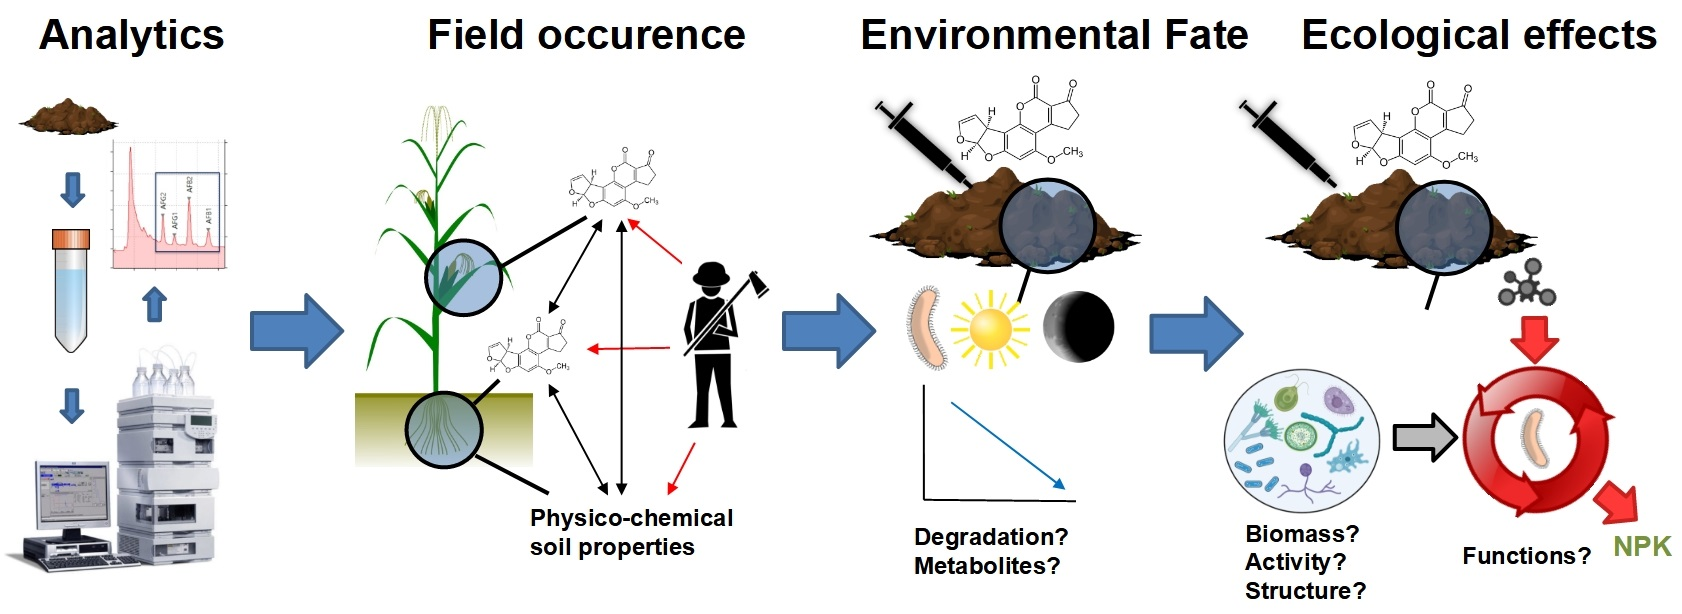
\includegraphics[width=1.125\textwidth,center]{figures/thesis structure.jpg}
\decoRule
\captionsetup{labelfont=bf, justification=raggedright, singlelinecheck=off, width=1.125\textwidth}
\caption{Graphical representation of the structure of the thesis.}
\label{fig:Thesis_structure}
\end{figure}
\afterpage{\FloatBarrier}
%++++++++++++++++++++++++++++++++++++++++++++++++++++++++++++++++++++++++++++++++++++++++


The first part (Chapter \ref{Chapter2}) describes the development and validation of an analytical methodology capable of reliably determining AFs in the soil environment. At the start of the PhD project, the lack of appropriate analytical methods to accurately quantify aflatoxins in soil posed a significant obstacle to adequately addressing the research questions and hypotheses. Therefore, I first started with the development and validation of analytical method aimed to be fast, simple, sensitive, and selective to allow for an effective analysis of the major relevant aflatoxins AFB1, AFB2, AFG1, and AFG2 in agricultural soil. The analytical method being developed for this PhD project emphasizes capacity building by avoiding the need for costly purification techniques like IAC cleanup and advanced instrumentation such as LC-MS, and instead utilizing HPLC-FLD for analysis (Chapter \ref{subchap:analysis}). My hypothesis is that by utilizing solvents with similar characteristics to aflatoxins, namely intermediate polarity and H-bond acceptor properties (Chapter \ref{subchap:analysis}), and incorporating an ultrasonication treatment during solvent extraction (USE) to reduce the size of soil agglomerates and clay minerals, the strong interactions between soil sorption sites (i.e. clay minerals and soil organic carbon) and AFs can be effectively overcome.


In the second part (Chapter \ref{Chapter3}), the previously validated method was then used to analyze real soil samples to identify conditions and agricultural practices leading to elevated AFs concentrations in soil. As part of the interdisciplinary and international project "AflaZ", a comprehensive field study was carried out during harvest season in a high-risk model region for Sub-Saharan Africa, namely Kenyan maize fields in the Makueni region. The investigation focused on whether various agricultural practices can effectively lower the concentration of AFs in fields. The implementation of innovative farming practices aimed in reducing the overall occurence of aflatoxigenic fungi and decrease the susceptibility of the crop plants to fungal infestation. These practices included: (1) push-pull farming, which involves planting repellent and pest-insect attracting plants to reduce overall insect damage to crops; (2) conservation tillage, which promotes beneficial soil organisms, improves plant health, and suppresses aflatoxigenic fungi; (3) the use of non-toxigenic and mycophagic \textit{Trichoderma} fungi, which preys on toxigenic \textit{Aspergillus} fungi; and (4) a control group that followed conventional farming practices, as typically practiced by the local population.


In the third part (Chapter \ref{Chapter4}), a laboratory incubation experiment was carried out to investigate the underlying degradation processes and their relationship with the physicochemical properties of the soil and available concentrations of AFs. In this regard, I aimed to simulate conditions, aflatoxins may be subjected to in fields. For this purpose, I designed a laboratory degradation experiment with two reference soils (clay and sandy loam) covering a range of soil properties, that are likely affecting the availability of AFs for the degradation processes, namely soil organic carbon and clay content. Non-sterile soils were incubated in dark to assess the microbial degration, while sterile soils functioned as a sterile control. Sterile soils were irradiated with UV light to simulate sunlight-induced photodegradation. Aflatoxin B1 was used as model compound, since it is the most frequently detected AFs in plant-based foods and feeds and due to the toxicological relevance. The samples were further analyzed for the formation of the previously described metabolites in soil matrices, i.e. AFB2, AFB2a, AFG1 and AFG2, thereby evaluating the transformation processes of AFB1.


In the fourth part (Chapter \ref{Chapter5}), I conducted a laboratory incubation experiment to evaluate the consequences of aflatoxin exposure to the soil microbiome and associated soil functions. To comprehensively evaluate the effects at different levels, including microbial responses in terms of biomass, activity, and catabolic functions (Chapter \ref{subsubchap:soilhealth_definitions}), I conducted an incubation study with two reference soils that exhibited a range of physicochemical properties and were artificially contaminated with AFB1 in an environmentally relevant range. To establish links to the findings from chapter 3, I employed the same reference soils, model compound, and concentrations.


Finally, in the concluding discussion (Chapter \ref{Chapter6}), I address the central hypothesis of this paper, explore in detail the implications of my findings, highlight new and unanswered questions and future perspectives, and explore possible research connections.
